\documentclass[book,openany]{jlreq}

\usepackage{graphicx}
\usepackage[pdfencoding=auto]{hyperref}
\usepackage{amsmath,amssymb,amsthm}
\usepackage{bm}
\usepackage{booktabs}
%\usepackage{subfig}
\usepackage{pifont}
\usepackage{url}
\usepackage{cite}
\usepackage{ulem}
\usepackage{siunitx}
%\usepackage{physics}
\usepackage{float}
\usepackage{tcolorbox}
\tcbuselibrary{breakable}
\usepackage{cancel}
\usepackage{color}
\renewcommand{\CancelColor}{\color{red}}

\theoremstyle{definition}
\newtheorem{theorem}{定理}[chapter]
\newtheorem*{theorem*}{定理}
\newtheorem{definition}[theorem]{定義}
\newtheorem*{definition*}{定義}

\usepackage{xcolor}
\hypersetup{
  bookmarksnumbered=true,
  colorlinks=true,
  citecolor=red,
  linkcolor=blue,
  urlcolor=orange,
}

\begin{document}
\title{\Large{SuperKEKBクライストロン電源の周辺}\\
    \normalsize{\textasciitilde 2023年度先任・主任技師による若手技術者のためのフォローアップ研修 \textasciitilde}}
\author{吉本 伸一}
\maketitle
\tableofcontents
\clearpage

\chapter{SuperKEKBのRFシステム}

\section{SuperKEKBのRFシステムの概要}

SuperKEKB加速器は4つの直線部を4つの弧で結んだレーストラック型で、4つの直線部のうちBelle II測定器がある筑波直線部を除いた3箇所と陽電子用のダンピングリングに電子、陽電子を加速するための高周波システムが配置されている。(図\ref{layout})にSuperKEKB加速器の高周波システムのレイアウトを示す。
%
\begin{figure}[!htt]
    \begin{center}
        \includegraphics[width=\linewidth]{figs/SKEKB-RF.pdf}
        \caption{Layout of SuperKEKB, showing the locations of RF buildings and RF stations.}
        \label{layout}
    \end{center}
\end{figure}

各RFステーションは、クライストロン、ハイパワーRFシステム(HPRF)、ローレベルRFシステム(LLRF)、RF空洞で構成される。(図\ref{layout})に示すように、ARESステーションでは、1台のクライストロンで2台の空洞を駆動する場合と、1台のクライストロンで1台の空洞を駆動する場合があるが、SCステーションでは1台のクライストロンで1つの空洞を駆動している。大穂(D4, D5)、富士(D7, D8)、日光(D10, D11)、ダンピングリングの四つの電源室に、電源1台で2本のクライストロンに電力を供給できるA型電源14台、電源1台で1本のクライストロンに電力を供給できるB型電源3台、計17台の電源設備があり、クライストロンは31本ある。電源装置は、できるだけ安価で安定した電源供給を目指したもので、殆どの電源が改良や老朽化対策を行いながら、設置から40年近く使い続けている。

電源とクライストロンは地上の電源室にありますが、そこから地下11 mにある周長3 kmの加速器トンネル内に加速空洞が設置されています。大穂と富士では常伝導空洞であるARES空洞が、日光では超伝導空洞が使われており、クライストロンから伸びた長い導波管でこれらの加速空洞へと繋がり、クライストロンから出た高周波電力が供給され、電子や陽電子を加速します。




\section{クライストロン電源の概要}

SuperKEKBのメインリング(MR)のクライストロン電源(KPS)には、2台のクライストロンに電源を供給するA型と、1台のクライストロンだけのB型が存在する。さらに、A型及びB型の半数は、交流\qty{6.6}{\kilo\volt}ラインの位相を\qty{15}{\degree}ずらしてあり、MRの電源室へ混在させて設置してある。これは、MRビームへのカソード電圧のリップルを通して影響、及び、逆に\qty{6.6}{\kilo\volt}ラインを通して中央変電所側への高次のノイズの発生等を考慮して行われた。つまり、カソード電圧は12相の全波整流でクローバ回路部にあるコンデンサーで平滑され、その半数は\qty{15}{\degree}位相がずれており、MR全体で見た場合大略、24相で整流されたものとみなせる見なせる。

電源は、各クライストロン1本につき、カソード、アノード/ヒータ、集東/補助集束コイルの電源から構成される 。A型電源では、カソード電圧は2本のクライ-ストロンで共通であるが、その他は独立に制御される。出力電圧はトランスの切替(無電圧時) によって、公称出力\qty{-50}{\kilo\volt}、\qty{-65}{\kilo\volt}、\qty{-80}{\kilo\volt}及び\qty{-90}{\kilo\volt}の内から1つ選択され、さらに微細な電圧調整は、可変範囲$\pm \qty{10}{\percent}$のIVRによって行われる。実際の運転においてはクライストロン負荷が変化しても、$\Delta Vk/Vk<\pm \qty{1}{\percent}$となる様にIVRを自動転している。各クライストロンへはカソード電庄\qty{-90}{\kilo\volt} でビーム電流\qty{20}{\ampere}まで供給可能である。アノード電源はコッククロフトワルトン型の電源で、カソード電位が基準電位なり、\qty{+80}{\kilo\volt}で\qty{10}{\milli\ampere}まで出力可能である。実際の運転においては、立下りを早めることが必要となり(後述)\qty{20}{\mega\ohm}の抵抗を外付けにクライストロンと並列にカソードとアノード間に挿入した。

\begin{figure}[!htt]
    \begin{center}
        \includegraphics[width=\linewidth]{figs/skeleton-diagram.pdf}
        \caption{Block diagram of a type-A KPS.}
        \label{f02-02}
    \end{center}
\end{figure}

\begin{figure}[!htt]
    \begin{center}
        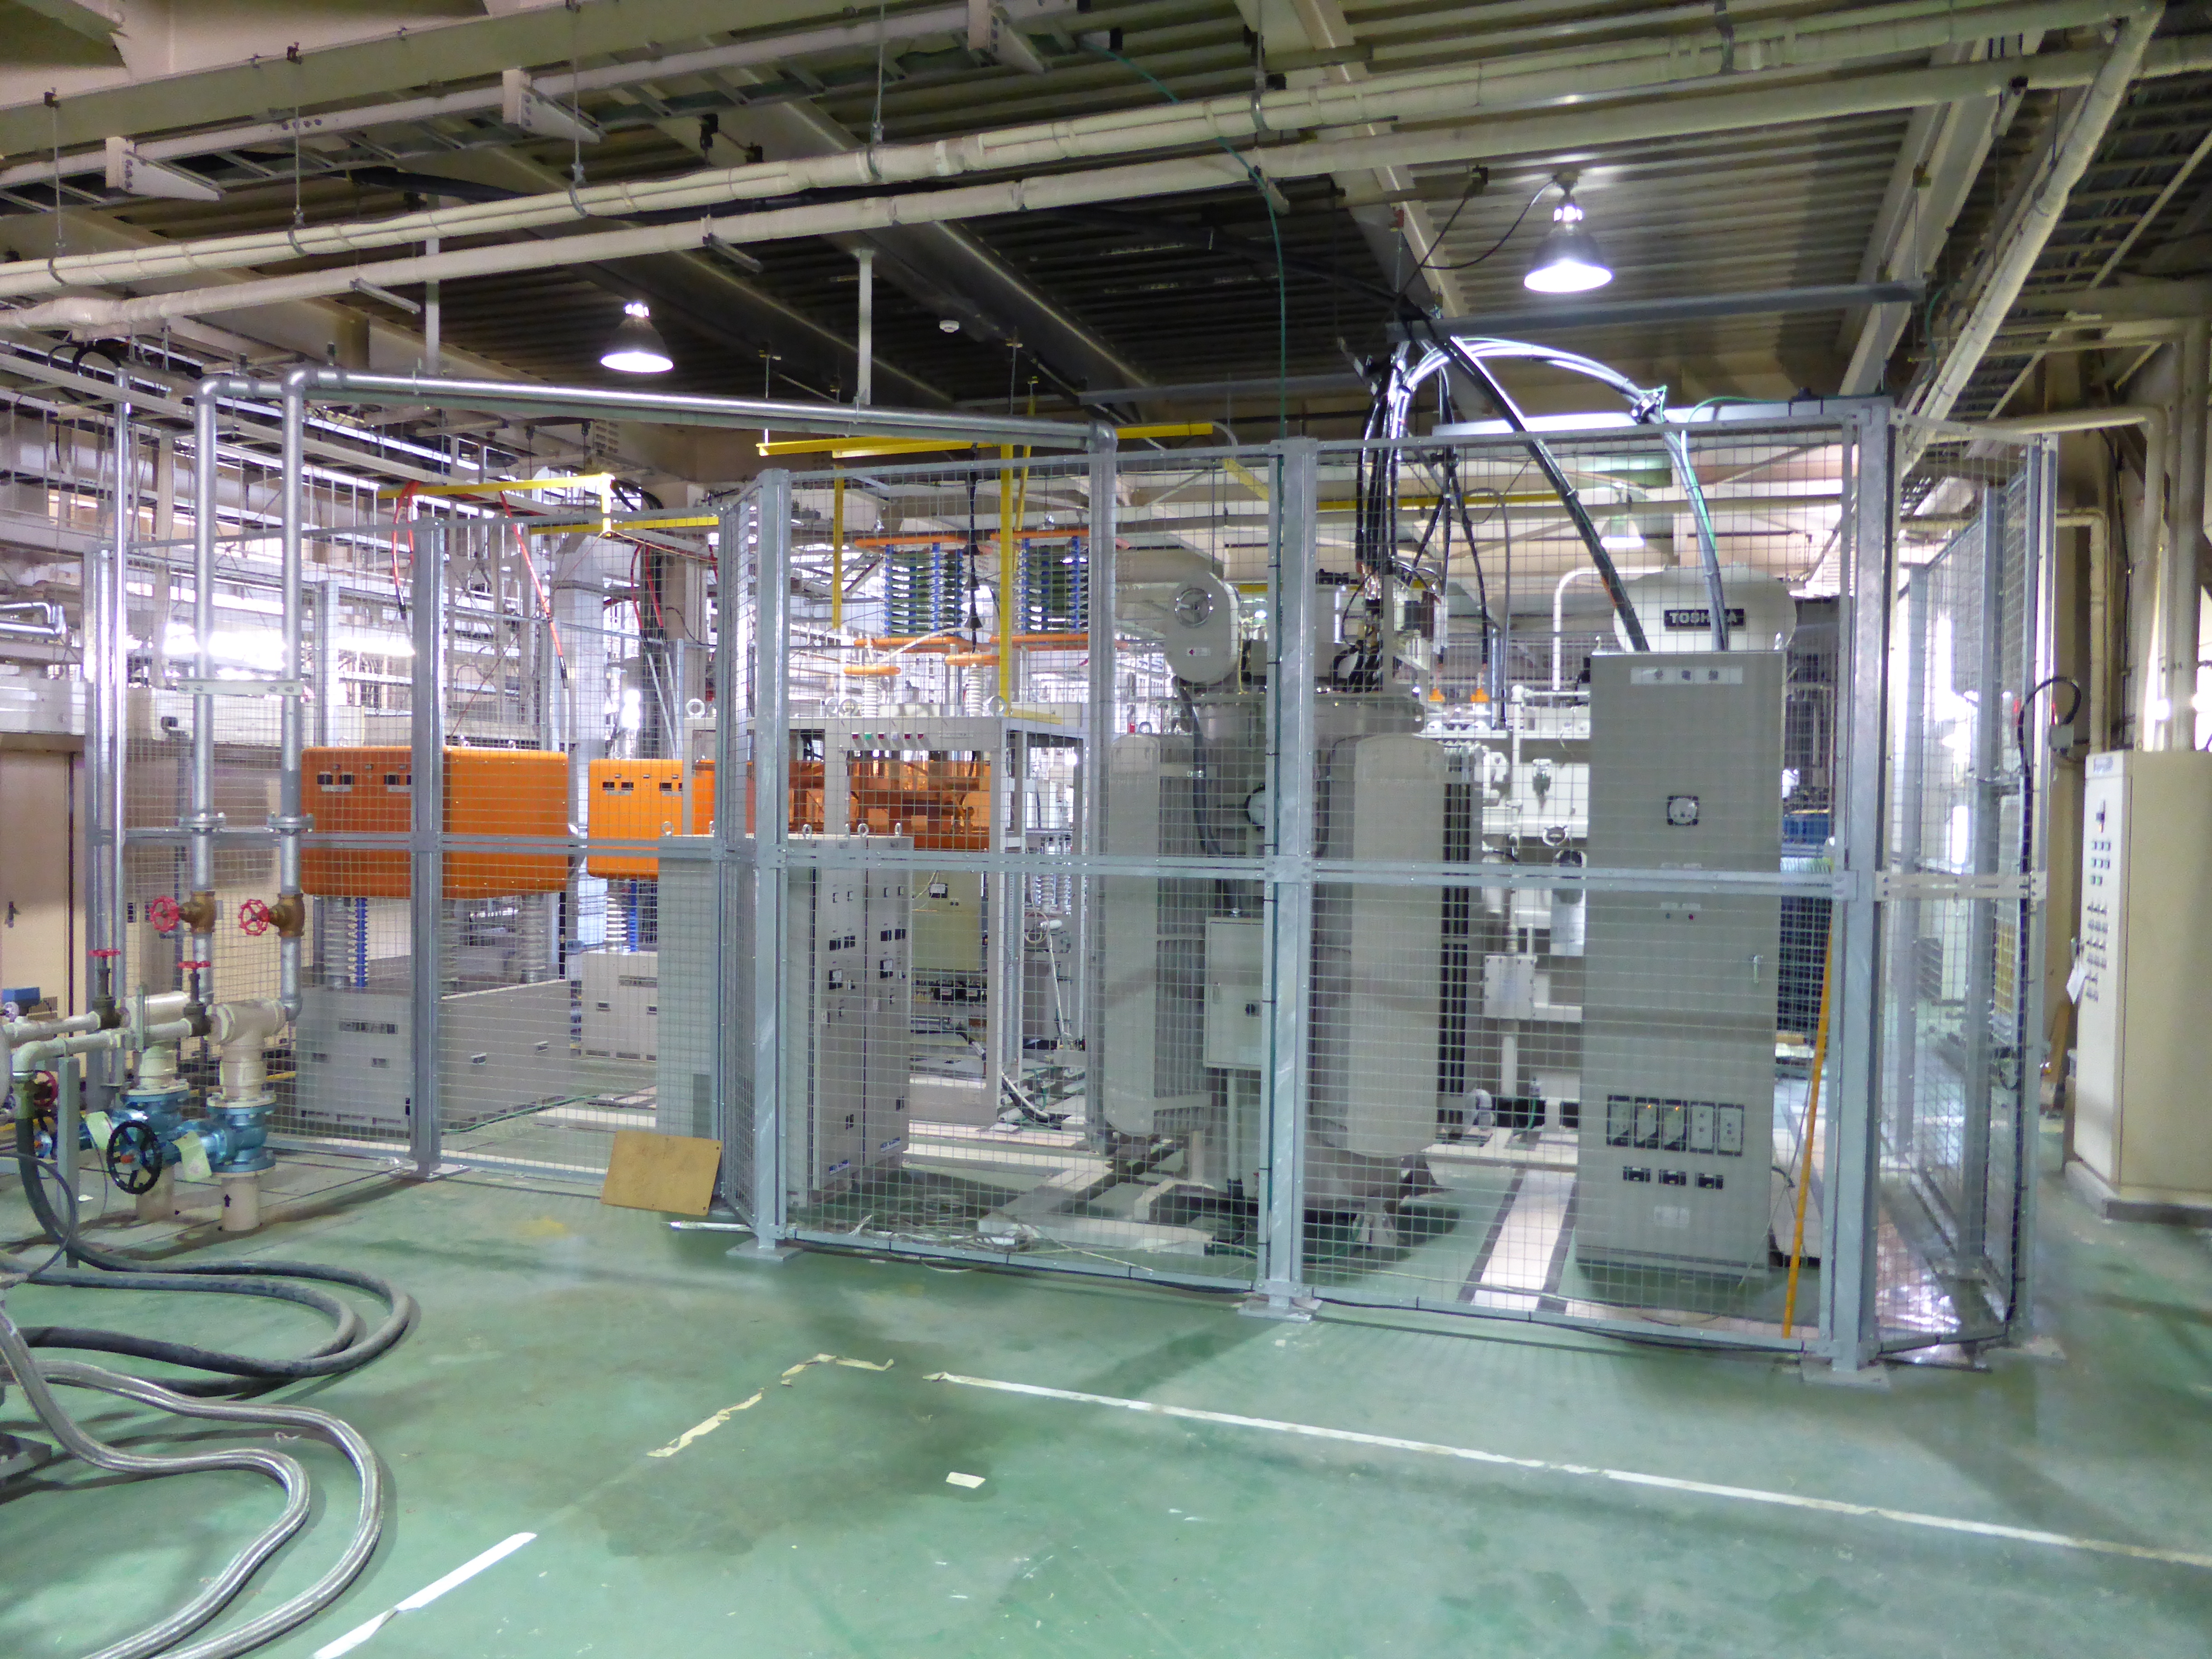
\includegraphics[width=\linewidth]{figs/KPS.JPG}
        \caption{クライストロン電源の全景}
        \label{kps_photo}
    \end{center}
\end{figure}

\subsection{直流高電圧カソード電源}
電源平滑コンデンサの容量を大きくすればするほど、リップル含有率は小さくなる。しかし、やみくもに大きくすれば良いという訳ではない。その理由は、電源投入時に平滑コンデンサを充電するために非常に大きな電流(突入電流)が流れてしまい、精密な回路を壊してしまう可能性があるからだ。したがって、充電時には$\mathrm{R_{SS}}$を直列に入れて突入電流を制限している。コンデンサが充電後はSSが閉じこの抵抗はバイパスされる。


\subsection{クローバースイッチ}
クライストロンを保護するためにクローバースイッチに要求される性能は、以下のようになる。

\begin{enumerate}
    \item カソード電圧が\SI{50}{\kilo\volt}以上の場合、負荷が短絡した時、クローバーは\SI{6}{\micro\second}以内に動作し、負荷へのエネルギー流入は\SI{30}{\joule}未満でなければならない。
    \item カソード電圧が\SI{30}{\kilo\volt}以下の場合、\SI{100}{\milli\second}以内に高圧を切ること。
\end{enumerate}

\SI{5}{\ohm}の抵抗がクライストロンのカソードとクローバースイッチの間に挿入されている。この抵抗は5本の直列に接続したイグナイトロンがトリガーするまでカソード電圧を保持するためにある。

\subsubsection{短絡試験}
\begin{figure}[!htt]
    \begin{center}
        \includegraphics[width=12cm,clip]{figs/sc_test.pdf}
        \caption{Block diagram of a type-A KPS.}
        \label{sctest}
    \end{center}
\end{figure}

\subsection{ヒーター・アノード電源}

\begin{figure}[!htt]
    \begin{center}
        \includegraphics[width=12cm,clip]{figs/anode_rise.png}
        \caption{Block diagram of a type-A KPS.}
        \label{anode}
    \end{center}
\end{figure}

\subsection{集束コイル電源}

\subsection{アースラインとノイズ}
\subsection{電源の制御とインターロック}

\begin{thebibliography}{9}
    \bibitem{Ono}
    M. Ono et al., TRISTAN RF system with normal conducting cavity, KEK Internal 87-6 (1987)
\end{thebibliography}
%
\end{document}